\documentclass[article]{stucosrec}

% for testing purposes only
\usepackage{lipsum}
\newcommand{\latex}{\LaTeX\xspace}

\title{\latex TEMPLATE FOR StuCoSReC CONTRIBUTION}
\author{
	Klemen Berkovi\v{c}\thanks{He did the most work} \\
	Faculty of Electrical \\Engineering and Computer Science,\\
	University of Maribor,\\
	Koro\v{s}ka cesta 46, 2000 Maribor, Slovenia \\
	\texttt{klemen.berkovic1@um.si} \\
	\And
	Iztok Fister Jr.\thanks{The best sponsor of them all} \\
	Faculty of Electrical \\Engineering and Computer Science,\\
	University of Maribor,\\
	Koro\v{s}ka cesta 46, 2000 Maribor, Slovenia \\
	\texttt{iztok.fister1@um.si} \\
	%% \And
	%% Coauthor \\
	%% Affiliation \\
	%% Address \\
	%% \texttt{email} \\
	%% \And
	%% Coauthor \\
	%% Affiliation \\
	%% Address \\
	%% \texttt{email} \\
}

% images directory
\imagespath{ {./images/} }

\begin{document}
	
	\maketitle
	
	\begin{abstract}
		\lipsum[1]
	\end{abstract}
		
	% keywords can be removed
	\keywords{First keyword \and Second keyword \and ...}
		
	\section{Introduction}
	\lipsum[2]
	\lipsum[3]
	
	
	\section{Headings: first level}
	\label{sec:headings}
	
	\lipsum[4] See Section \ref{sec:headings}.
	
	\subsection{Headings: second level}
	\lipsum[5]
	
	\subsubsection{Headings: third level}
	\lipsum[6]
	
	\paragraph{Paragraph}
	\lipsum[7]	
	
	\section{Examples of citations, figures, tables, references}
	\label{sec:others}
	
	\subsection{Citations}
	Citations use \verb+natbib+. The documentation may be found at
	\begin{center}
		\url{http://mirrors.ctan.org/macros/latex/contrib/natbib/natnotes.pdf}
	\end{center}
	
	Here is an example usage of the two main commands (\verb+citet+ and \verb+citep+)~\cite{vrbancic2019transfer}.
	
	\subsection{Figures}
	\lipsum[10]
	See Figure~\ref{fig:fig1}. Here is how you add footnotes. \footnote{Sample of the first footnote.}
	\lipsum[11]
	
	\begin{figure}[H]
		\centering
		\fbox{\rule[-.5cm]{4cm}{4cm} \rule[-.5cm]{4cm}{0cm}}
		\caption{Sample figure caption.}
		\label{fig:fig1}
	\end{figure}

	See Figure~\ref{fig:fig2}. This is an example of pdf image.

	\begin{figure}[b!]
		\centering
		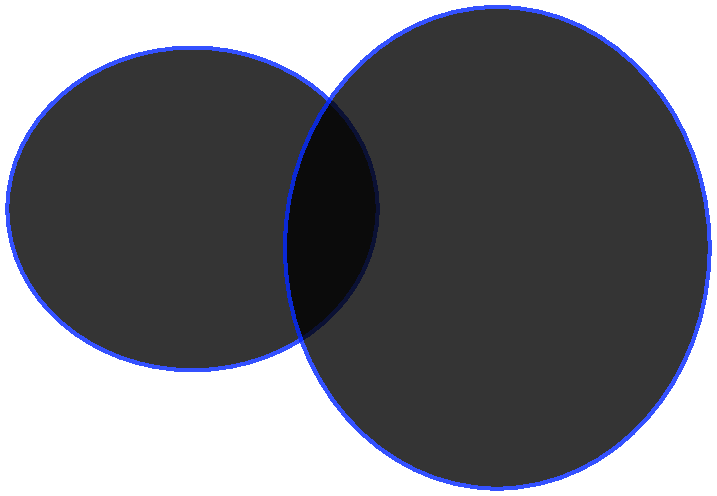
\includegraphics[scale=.5]{drawingOne.pdf}
		\caption{Sample figure caption.}
		\label{fig:fig2}
	\end{figure}

	See Figure~\ref{fig:fig3}. This is an example of png image.
	
	\begin{figure}[H]
		\centering
		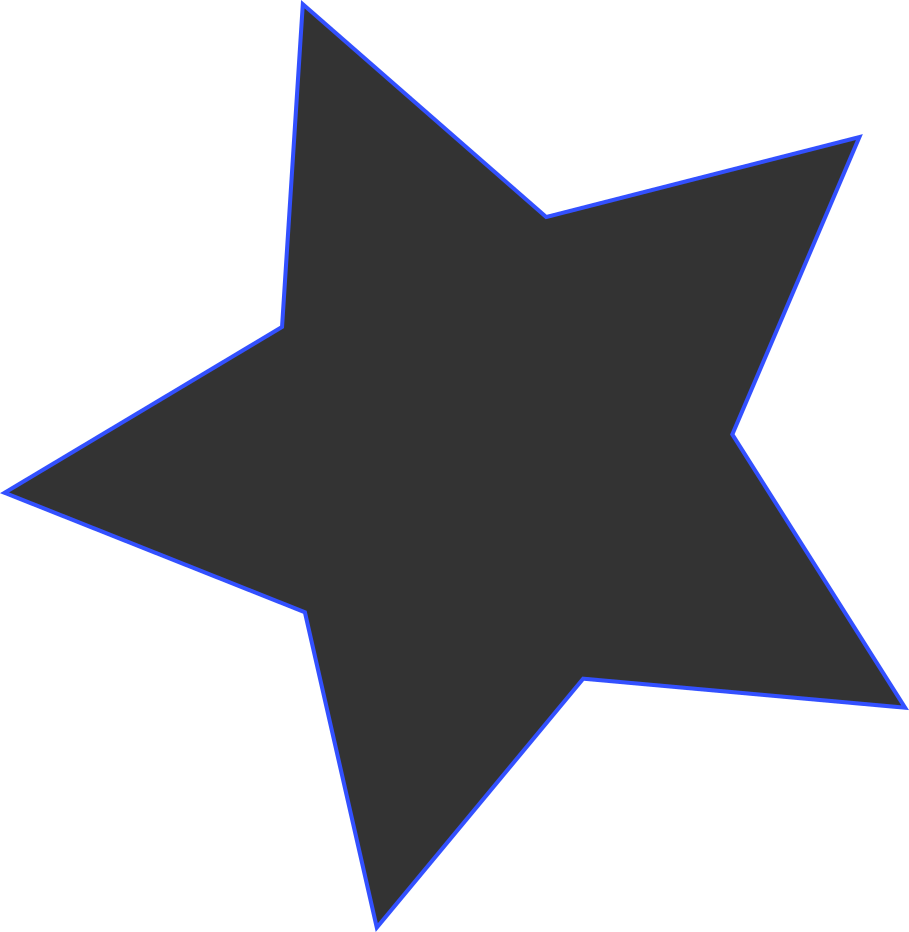
\includegraphics[scale=.5]{drawingTwo.png}
		\caption{Sample figure caption.}
		\label{fig:fig3}
	\end{figure}

	\subsection{Tables}
	See awesome Table~\ref{tab:table}.
	
	The documentation for \verb+booktabs+ (`Publication quality tables in LaTeX') is available from:
	\begin{center}
		\url{https://www.ctan.org/pkg/booktabs}
	\end{center}	
	
	\begin{table*}
		\centering
		\caption{Some Typical Commands}
		\label{tab:table}
		\begin{tabular}{|c|c|l|} \hline
			Command&A Number&Comments\\ \hline
			\texttt{{\char'134}alignauthor} & 100& Author alignment\\ \hline
			\texttt{{\char'134}numberofauthors}& 200& Author enumeration\\ \hline
			\texttt{{\char'134}table}& 300 & For tables\\ \hline
			\texttt{{\char'134}table*}& 400& For wider tables\\ \hline
		\end{tabular}
	\end{table*}

	\begin{table}[H]
		\centering
		\caption{Frequency of Special Characters}
		\begin{tabular}{|c|c|l|} \hline
			Non-English or Math&Frequency&Comments\\ \hline
			\O & 1 in 1,000& For Swedish names\\ \hline
			$\pi$ & 1 in 5& Common in math\\ \hline
			\$ & 4 in 5 & Used in business\\ \hline
			$\Psi^2_1$ & 1 in 40,000& Unexplained usage\\
			\hline
		\end{tabular}
	\end{table}
	
	\subsection{Lists}
	\begin{itemize}
		\item Lorem ipsum dolor sit amet
		\item consectetur adipiscing elit.
		\item Aliquam dignissim blandit est, in dictum tortor gravida eget. In ac rutrum magna.
	\end{itemize}

	\section{Math Equations}
	You may want to display math equations in three distinct styles:
	inline, numbered or non-numbered display.  Each of
	the three are discussed in the next sections.
	
	\subsection{Inline (In-text) Equations}
	A formula that appears in the running text is called an
	inline or in-text formula.  It is produced by the
	\textbf{math} environment, which can be
	invoked with the usual \texttt{{\char'134}begin. . .{\char'134}end}
	construction or with the short form \texttt{\$. . .\$}. You
	can use any of the symbols and structures,
	from $\alpha$ to $\omega$, available in
	\LaTeX\cite{Lamport:LaTeX}; this section will simply show a
	few examples of in-text equations in context. Notice how
	this equation: \begin{math}\lim_{n\rightarrow \infty}x=0\end{math},
	set here in in-line math style, looks slightly different when
	set in display style.  (See next section).
	
	\subsection{Display Equations}
	A numbered display equation -- one set off by vertical space
	from the text and centered horizontally -- is produced
	by the \textbf{equation} environment. An unnumbered display
	equation is produced by the \textbf{displaymath} environment.
	
	Again, in either environment, you can use any of the symbols
	and structures available in \LaTeX; this section will just
	give a couple of examples of display equations in context.
	First, consider the equation, shown as an inline equation above:
	\begin{equation}\lim_{n\rightarrow \infty}x=0\end{equation}
	Notice how it is formatted somewhat differently in
	the \textbf{displaymath}
	environment.  Now, we'll enter an unnumbered equation:
	\begin{displaymath}\sum_{i=0}^{\infty} x + 1\end{displaymath}
	and follow it with another numbered equation:
	\begin{equation}\sum_{i=0}^{\infty}x_i=\int_{0}^{\pi+2} f\end{equation}
	just to demonstrate \LaTeX's able handling of numbering.
	
	\subsection{One more example}
	When $a \ne 0$, there are two solutions to $ax^2 + bx + c = 0$ and they are
	$$x = {-b \pm \sqrt{b^2-4ac} \over 2a}.$$
	
	\bibliography{references}

\end{document}
